En este capítulo se explican de forma precisa y justificada los distintos métodos seguidos 
en este problema, así como la presentación de un esquema del desarrollo. Para ello, se expone 
primeramente la contextualización avanzada del problema en cuestión a resolver, seguido de la 
explicación de las distintas etapas que constituyen el trabajo. Posteriormente, se mencionan 
las distintas herramientas que se usan en este proyecto.

\section{Definición del problema}
\label{section:problem_def}
Este trabajo se realiza dentro de la Cátedra 
\textit{Inteligencia Artificial para el Transporte y Movilidad}\footnote{La UC3M y 
EMT Madrid presentan una nueva Cátedra en Inteligencia Artificial para el transporte y 
la movilidad \url{https://www.uc3m.es/ss/Satellite/UC3MInstitucional/es/Detalle/Comunicacion_C/1371438766717/1371216001122/La_UC3M_y_EMT_Madrid_presentan_una_nueva_Catedra_en_Inteligencia_Artificial_para_el_transporte_y_l} 
(accedido: 6 de mayo de 2026).}. Esta establece un nexo colaborativo entre la EMT y la Universidad 
a través del grupo de investigación GIAA\footnote{(Grupo de Inteligencia Artificial Aplicada) 
\url{https://giaa.uc3m.es/} (accedido: 6 de mayo de 2026).}. Como se explica de forma breve en 
la introducción, La Empresa Municipal de Transportes propone estudiar la viabilidad de la construcción 
de un sistema para analizar el rendimiento de rutas de autobuses. El principal motivo detrás de este 
planteamiento es la falta de un simulador propio para realizar esta tarea, que se suma a la existencia 
de  una entidad superior a la EMT, el CRTM( Consorcio Regional de Transportes de Madrid) 
\footnote{\url{https://www.crtm.es/}  (accedido: 6 de mayo de 2026)}, que se encarga de validar 
diariamente las dotaciones propuestas por la compañía de autobuses. La \enquote{caja negra} que 
implica este paso para la validación supone un componente extra que justifica esta propuesta. La 
realización de este proyecto se ha enmarcado en un trabajo de investigación de una duración de ocho 
meses a lo largo de los cuales se ha ido desarrollando la solución planteada, bajo la supervisión 
bisemanal por parte de la EMT mediante reuniones telemáticas.

En una fase de desarrollo inicial, se propuso por parte de la EMT la evaluación de las cinco 
líneas \textit{express} de la compañía, al ser líneas con un número de paradas bajo relativo al 
general de las rutas. Esta distinción permite acotar el análisis previo a la simulación, necesario para 
la validación de la viabilidad del simulador.

Una de las decisiones más relevantes para la comprensión del alcance de este trabajo es la 
de simular el comportamiento únicamente de los \textbf{días normales de operación}, excluyendo
datos relativos a festividades, cambios de estacióno eventos de gratuidad promovidos por la compañía. 
Los distintos motivos detrás de esta decisión se enuncian en la sección \ref{section:gauss_and_study} 
y posibles variaciones de este análisis se discuten en el capítulo \ref{chapter:future_works}.

Para la utilización de datos reales, la EMT puso a disposición una base de datos relacional 
con los datos de operación de las paradas de las líneas Express desde el 1 de julio de 2025, con 
actualizaciones diarias, permitiendo ir ampliando la base que compone el análisis a medida que se iba 
completando.

\section{Estructura de trabajo}
\label{subsec:structure}
El proyecto se puede separar en cuatro partes características. A continuación, se expone cada 
una con ---Nombre, Duración, Explicación de contenido---. En la figura \ref{fig:gantt_diagram} se 
puede ver, representado a modo de diagrama de \textit{Gantt}, las distintas fases espaciadas en el 
tiempo.

\begin{itemize}

\item \textbf{Investigación y Planteamiento}: Duración [6 semanas]

Supone la fase inicial del trabajo. Al no disponer de los datos, expandidos en el capítulo
 \ref{chapter:param_analisys}, y debido a la naturaleza investigadora del trabajo, en una primera 
 etapa, se realizó un análisis del estado de la cuestión, expuesto en la 
 sección \ref{chapter:state_of_art}, junto con un estudio de la plataforma 
 GAMA~\cite{taillandier2019gama}, con el fin de realizar un acercamiento a los conceptos, 
 estándares y herramientas que se usan a lo largo del desarrollo. Durante esta fase, a lo 
 largo de las reuniones bisemanales, se acota el rango de aplicación del simulador, reduciéndose 
 de las cinco líneas express inicialmente deseadas, a la línea E01, con el fin de no sobrecargar el 
 análisis de la fase posterior.

\item \textbf{Análisis y Parametrización de Datos}: Duración [12 semanas]

En esta etapa se realiza un estudio exhaustivo sobre los datos facilitados, tanto los datos 
geoespaciales de la ruta, como los datos de operación de los autobuses. A lo largo de estas doce 
semanas, se procesa esta información para analizar la viabilidad de la solución planteada durante la 
fase uno, basándose en criterios estrictos de modelado de distribuciones para los distintos parámetros 
que sirven de entrada al simulador.

\item \textbf{Diseño e Implementación en GAMA}: Duración [14 semanas]

Una vez estudiada la viabilidad de usar los datos de operación de autobuses y preparados los 
parámetros de entrada al simulador, en esta etapa se construye la arquitectura del sistema 
multiagente y su desarrollo en el lenguaje propio de GAMA \enquote{GAML} \cite{taillandier2019gama}. 
A lo largo de esta fase, expandida posteriormente, 
se construyen dos modelos distintos: uno en el que los pasajeros se representan como agentes 
individuales con comportamiento propio, y otro en el que las subidas y bajadas se modelan de 
forma agregada por parada, priorizando el rendimiento computacional de la simulación.

\item  \textbf{Extracción de indicadores y visualización}: Duración [5 semanas]

En esta última fase, se parte del simulador prácticamente completado, y se construye una 
herramienta de visualización y de lanzamiento en local de los distintos escenarios que plantee 
el usuario. Por otra parte, se completa el simulador con el feedback de formato de datos que 
requiere el extractor de KPIs.


\end{itemize}

\clearpage

\begin{landscape}
\thispagestyle{landscape}
\begin{figure}[H]
 \centering
    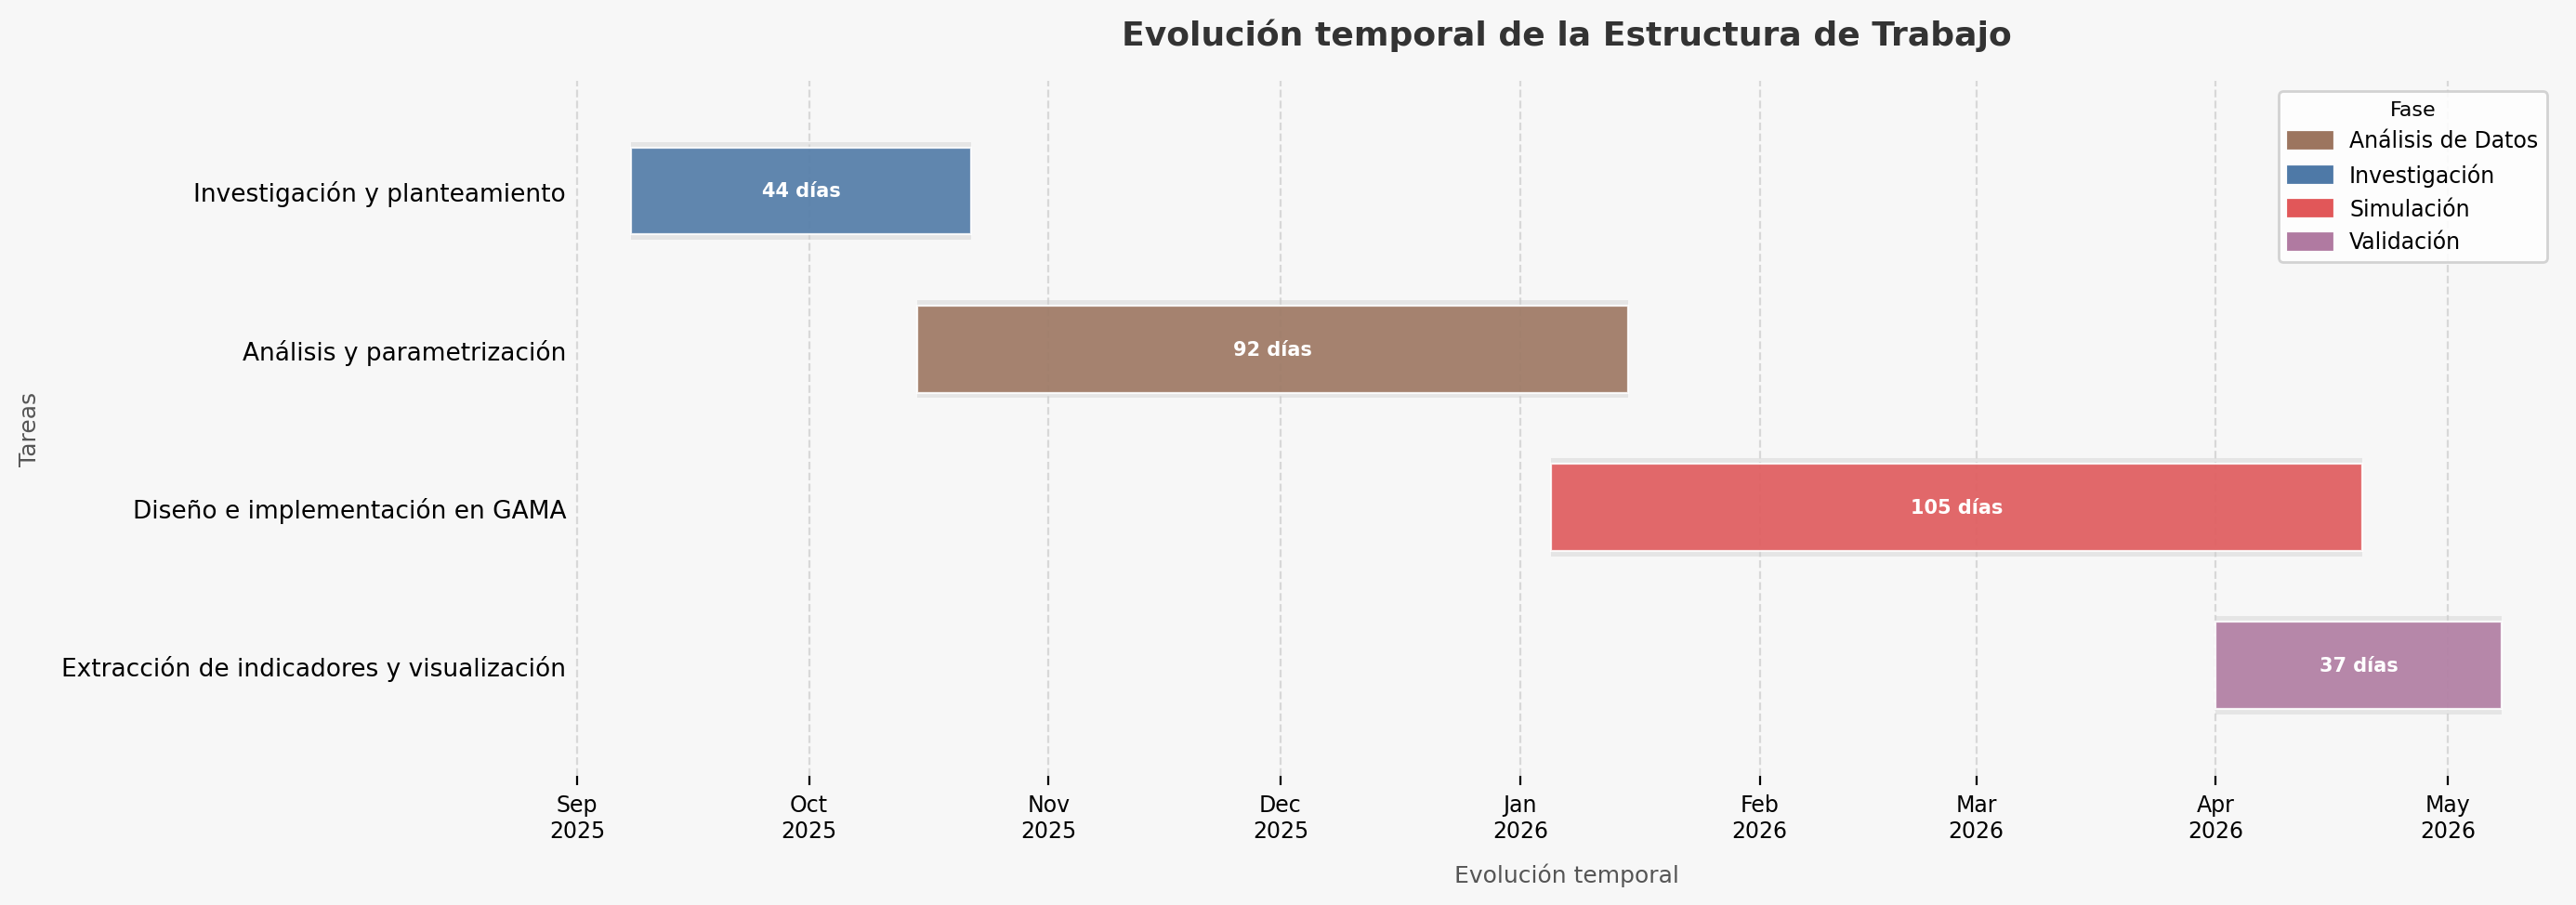
\includegraphics[width=0.9\textwidth,height=0.5\textheight]{imagenes/gantt_chart.png}
\caption{Diagrama de Gantt explicativo relativo a las distintas fases del desarrollo}
\par\vspace{4pt}{\footnotesize Fuente: Elaboración propia.}
\label{fig:gantt_diagram}
\end{figure}

\end{landscape}
\afterpage{
    \null
    \thispagestyle{plain}
}

\section{Herramientas Utilizadas}
En esta sección se exponen las distintas herramientas utilizadas para la construcción del sistema, junto a una breve explicación de su peso en ella.


\begin{itemize}


\item \textbf{GAMA}:
Usada en el desarrollo del sistema multi-agente, facilita la implementación del estándar de comunicaciones FIPA~\cite{fipa2002acl} y la inclusión de mapas geoespaciales. 

\item \textbf{Jupyter Notebook}\footnote{\url{https://jupyter.org} (accedido: 9 de mayo de 2026).}:
Herramienta usada con kernel de \textit{Python} para el análisis de los datos de operación de la línea a simular. Facilita la visualización de resultados, el análisis exploratorio de datos o la construcción de modelos estadísticos. Con  su estructura de celdas \enquote{markdown} y sus celdas de código, mejora la lectura y la explicabilidad de los procesos que se realizan en cada documento \enquote{ipynb} (formato de cuadernos Jupyter).

\item \textbf{QGIS}\footnote{\url{https://qgis.org} (accedido: 9 de mayo de 2026).}:
Necesaria para la conversión de GeoJSON (Formato basado en JSON con especificación concreta de parámetros para representación geográfica de los datos) a archivo ESRI shapefile (formato estándar de representación vectorial de datos geoespaciales) . Usada para la carga en el simulador de los datos de la ruta y de la ubicación de las paradas.

\item \textbf{Node.js}\footnote{\url{https://nodejs.org} (accedido: 9 de mayo de 2026).}:
Framework de desarrollo web utilizado para el despliegue de la herramienta en \textit{local}. Permite la creación de una arquitectura cliente/servidor que permita la conexión entre acciones o deseos del usuario en el navegador y su correspondiente cambio en la máquina anfitriona. Facilita la visualización de las simulaciones o el lanzamiento de nuevas.

\item \textbf{Docker}\footnote{\url{https://www.docker.com} (accedido: 9 de mayo de 2026).}:
Usado para la estandarización y aislamiento de procesos, facilitando el uso global del sistema. Utilizado para el despliegue de un contenedor encargado de la ejecución del programa completo, emulando un \enquote{gemelo digital} con las características del ordenador utilizado para el desarrollo. Gracias a esta herramienta, se permite ejecutar simulaciones en entornos sin la plataforma de desarrollo de agentes instalada.

\item \textbf{Python}\footnote{\url{https://www.python.org} (accedido: 9 de mayo de 2026).}:
Lenguaje de programación usado para la extracción de métricas de rendimiento de las distintas simulaciones. Sus librerías diseñadas para análisis de datos sobre grandes volúmenes como puede ser el caso de \textit{pandas} o generación de gráficas concretas con \textit{matplotlib} permiten generar estas KPIs con mayor facilidad.

\end{itemize}

Sobre las herramientas físicas utilizadas, se ha dispuesto de un portátil MSI Modern 15 C13M-273XES, 
modelo con 16 núcleos lógicos, 32GB RAM DDR4 y almacenamiento NVMe. Esta información, junto a detalles sobre presupuesto, 
se expanden en el capítulo \ref{chapter:budget}, pero cabe ser destacada por su relación a las herramientas usadas 
y su interés en la interpretación a nivel de tiempo en la fase de \textbf{Diseño
e implementación}, así como en la relativa a \textbf{Extracción de indicadores y visualización}.

Todo el desarrollo del trabajo se ha realizado sobre el sistema operativo Ubuntu 24.04 LTS, distribución 
de Linux basada en Debian. Esta elección de Sistema Operativo, sumado al conjunto de herramientas utilizadas,
 constituye un sistema de \textbf{código abierto} en su totalidad. Esto permite un sistema transparente y reproducible, 
 sin dependencia de licencias comerciales.